\section{付録}
  \label{付録}
    \subsection{ESP32 DEVKIT V1のピン番号レイアウト}
      \label{sec:ESP32 DEVKIT V1のピン番号レイアウト}
        \begin{figure}[htbp]
          \centering
          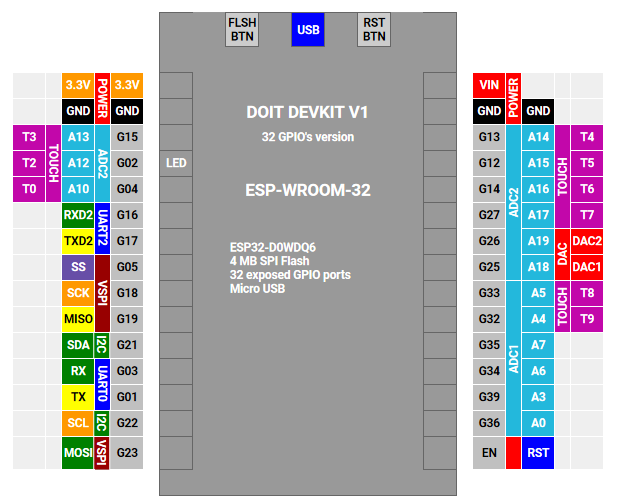
\includegraphics[scale=1]
          {figures/DOIT-DEVKIT-V1-32.png}
          \caption{ESP32 DEVKIT V1のピン番号レイアウト,Tim Sinaeve,beNative/ESP32-GPIO-list: ESP32 pinouts,DOIT modules in README.md.\cite{esppingithub}より引用}
          \label{fig:ピン番号レイアウト}
        \end{figure}
  
       \subsection{ソースコード}
        \label{sec:ソースコード}
         \par 別途,CD-ROMに実験に用いた全てのソースコードを添付する.具体的なディレクトリやコードの説明はルートディレクトリに保存するREADME.mdファイルを参照されたい.

       \subsection{API仕様書}
        \label{sec:API仕様書}
         \par 本研究で構築したAPI仕様書を添付する.ただし,ソースコードからローカルサーバを立ち上げ,ブラウザで表示させることでデバッグすることも可能であるため,そちらを推奨する.
    
       \subsection{情報処理学会予稿}
        \label{情報処理学会予稿}
         \par 別途,情報処理学会の発表内容の予稿を添付する.

       \subsection{紀要論文}
        \label{紀要論文}
         \par 別途,紀要論文を添付する.
    % \subsection{機械学習モデルの設計}
    %   \label{sec:machine_learning_model_design}
    %     \par

    % \subsection{機械学習モデルの実装}
    %   \label{sec:機械学習モデルの実装}
    %    \par 
      
    %   \subsubsection{データセットの準備}
    %     \label{sec:データセットの準備}
    %       \par
          
    %   \subsubsection{特徴量の選択と前処理}
    %     \label{sec:特徴量の選択と前処理}
    %       \par
          
    %   \subsubsection{モデルの学習と評価}
    %     \label{sec:モデルの学習と評価}
    %       \par
          
    % \subsection{機械学習モデルの結果分析}
    %   \label{sec:機械学習モデルの結果分析}
    %     \par
